\documentclass[a4paper, 12pt, titlepage]{article}

\usepackage{graphicx, color} %for å inkludere grafikk
\usepackage{verbatim, color} %for å inkludere filer med tegn LaTeX ikke liker. \verbatiminput{verb.txt}
%\usepackage{gensymb} %gensymb Symbols Defined to Work in Both Math and Text Mode 

\usepackage[T1]{fontenc} %for å bruke æøå. upgrades to 256 bit encoding. More characters
\usepackage[utf8]{inputenc} %Kan forandres til latin1. utf8 gir norske tegn
%inputenc allows the user to input accented characters directly from the keyboard;
%fontenc is oriented to output, that is, what fonts to use for printing characters.
%\usepackage[norsk]{babel} 

\usepackage{pdfpages} %Importing external pdf-pages
\usepackage[compact]{titlesec} %Spacing for two-column document

\usepackage{textcomp} % make degrees centigrade symbols, euros, etc
\usepackage{amsmath, amssymb} %e.g. \begin{theorem}[Pythagoras], \begin{proof} or {align}
\usepackage{amsbsy, amsfonts} %\pmb for annerledes boldfont
\usepackage{parskip} %Space between paragraphs
\usepackage{float} %Im­proves the in­ter­face for defin­ing float­ing ob­jects such as fig­ures and ta­bles.
\usepackage{simplewick}
\usepackage{libertine} 
\usepackage{siunitx} % SI units. Example: \SI{100}{\micro\meter}

\usepackage{geometry} % Definerer marger. 
 %\geometry{headhight=1mm}
 \geometry{top=20mm, bottom=20mm, left=34mm, right=34mm} % Marger i mm. Total bredde er 210mm



\author{Wilhelm Holmen}
\title{FYS4411 Project 1}

\begin{document}
 \maketitle
 \newpage

 \section*{1a}
 In this exercise I will use Monte Carlo integration to compute the expectation value for the energy. 
 \begin{align*}
 	\left< E \right> = \frac{\int d \mathbf{r_1} d \mathbf{r_2} \psi_T^*(r_1,r_2) \hat H \psi_T(r_1,r_2)}{\int d \mathbf{r_1} d \mathbf{r_2} \psi_T^*(r_1,r_2) \psi_T(r_1,r_2)}
 \end{align*}
 I need a wavefunction for this, so first I choose the ground state wavefunction solution the hydrogen atom, $e^{-\alpha r}$, for both the particles. This gives the total wavefunction
 \begin{align*}
 	\Psi_T(r_1,r_2) = e^{-\alpha(r_1 + r_2)}
 \end{align*}
 This is not the correct wavefunction, but it can give a decent first evaluation. 

 In the Metropolis algorithm, I will check wether a move given by, $\mathbf{R^{'}} = \mathbf{R} + \delta \cdot r $, will be accepted. $r$ is a random number in $[0,1]$. The acceptance criteria is given by
 \begin{align*}
 	\frac{P(\mathbf{R^{'}} )}{P(\mathbf{R} )} = \frac{\int d \mathbf{R^{'}} \psi^*_T(\mathbf{R^{'}} ) \psi_T(\mathbf{R^{'}} )}{\int d \mathbf{R} \psi^*_T(\mathbf{R}) \psi_T(\mathbf{R} )} \geq r
 \end{align*}

 Because of the variational princible, the trial energy will always be higher than the true energy. Therefore we can adjust $\alpha$ and the steplength $\delta$ until we get the lowest possible energy. The best steplength $\delta$ is a steplength that will accept around $50\%$ of the proposed steps. Using an algorithm that loops over different steplengths, I adjust $\alpha$ and plot the energy and variance as a function of $\alpha$. I start the steplength at $\delta = 1.2$ and increase it by $0.5*r$, $r \in [0,1]$ for each step. Testing if the number of accepted steps are within $[0.49,0.51]$ I either accept the step length or increase it.  

 \begin{figure}[H]
 	\centering
 	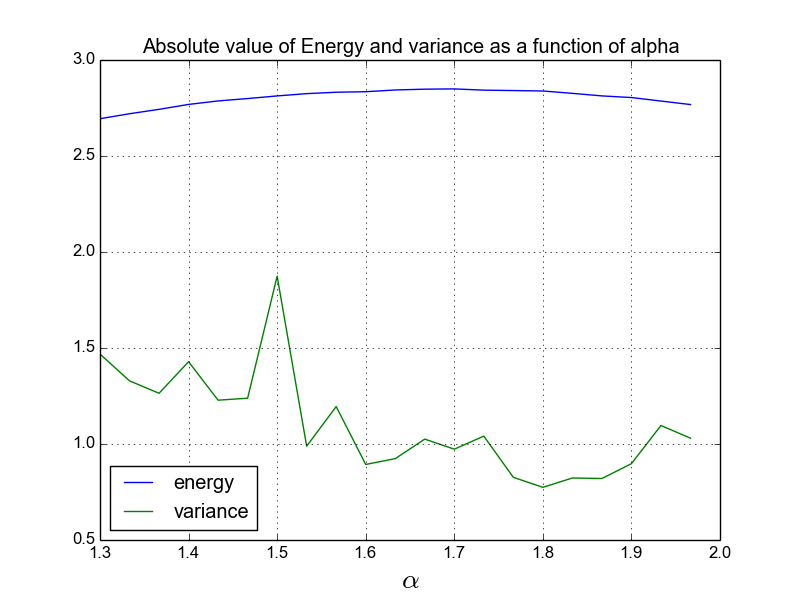
\includegraphics[width=\textwidth]{../python_programs/EnergyVariance_helium1.png}
 \end{figure}

 By looking closer at the energy and variance around $\alpha = 1.68$, we see that we get an energy of $\left<E\right> = -2.84997$, with a variance of $\sigma ^2 = 0.932912$. This is pretty close to the real value of $E_{exact} = -2.903$. We see however that the variance is smaller for $\alpha = 1.8$, $1.9$ and $1.6$.
 
 \begin{figure}[H]
 	\centering
 	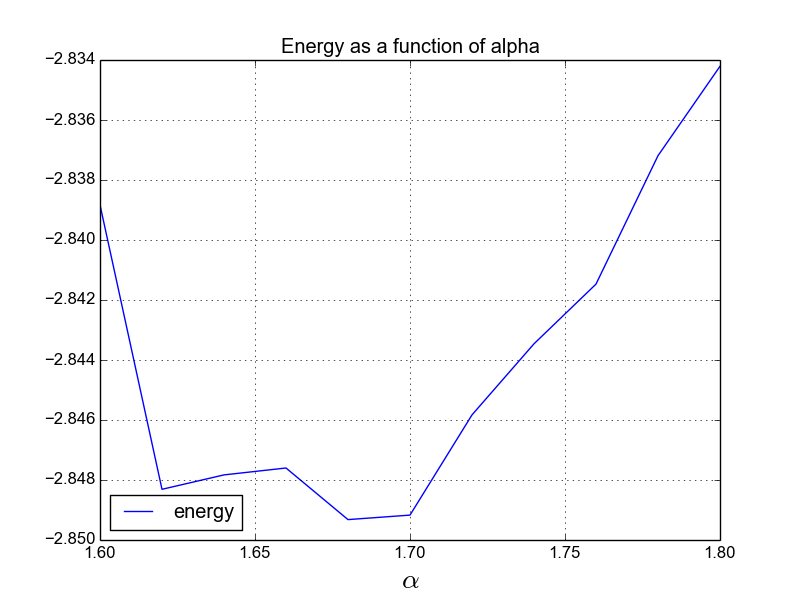
\includegraphics[width=\textwidth]{../python_programs/EnergyVariance_helium2.png}
 \end{figure}

 \begin{figure}[H]
 	\centering
 	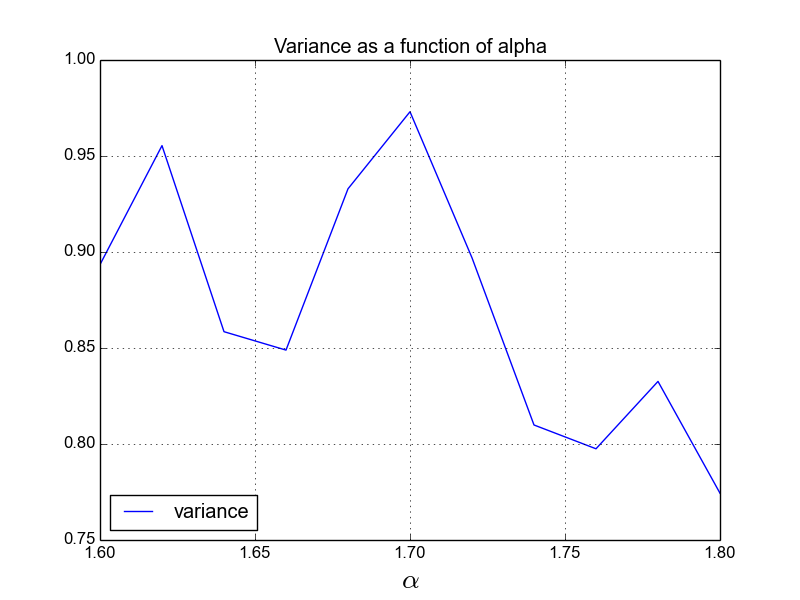
\includegraphics[width=\textwidth]{../python_programs/EnergyVariance_helium3.png}
 \end{figure}

 We can get a better result by improving our test function, $\Psi_T$. We can introduce a Jastrow factor. Here $r_{12} = |r_1 - r_2|$. 
 \begin{align*}
 	\Psi_T(r_1,r_2) = e^{-\alpha(r_1 + r_2)}e^{\frac{r_{12}}{2(1+\beta r_{12})}}
 \end{align*}
 
 Setting $\beta = 1.0$, we see that we can achieve a better energy, namely $\left<E\right> = -2.88013$. 
 \begin{figure}[H]
 	\centering
 	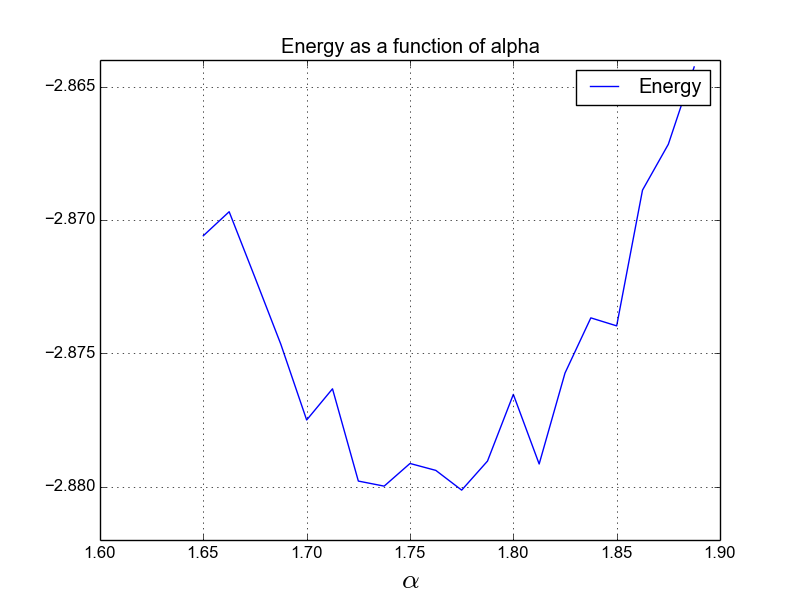
\includegraphics[width=\textwidth]{../python_programs/EnergyVariance_helium4.png}
 \end{figure}
 \begin{figure}[H]
 	\centering
 	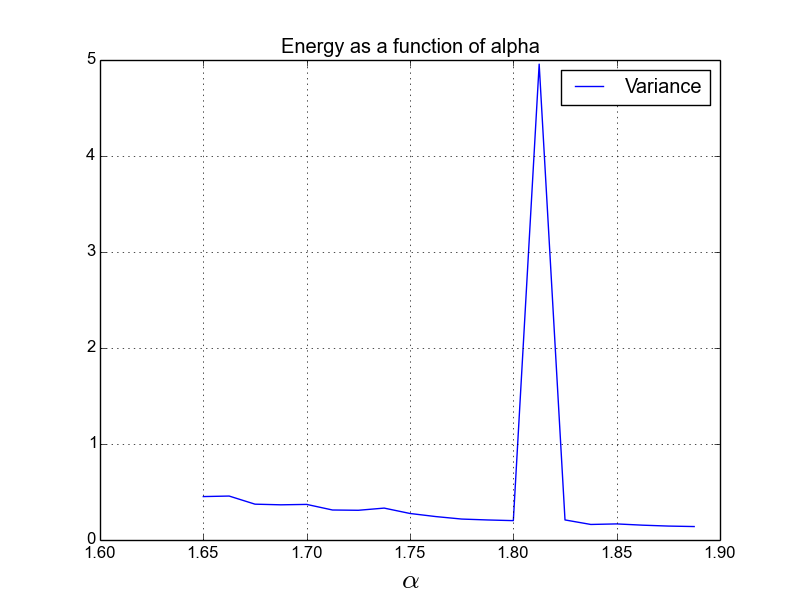
\includegraphics[width=\textwidth]{../python_programs/EnergyVariance_helium5.png}
 \end{figure}

\section*{b}
\begin{align*}
	\Psi_T &= e^{-\alpha(r_1 + r_2)} \\
	E_L &= \frac{1}{\Psi_T} \hat H \Psi_T \\
	\hat H &= -\frac{1}{2}\nabla_1^2 - \frac{1}{2}\nabla_2^2 - \frac{2}{r_1} - \frac{2}{r_2} + \frac{1}{r_{12}} \\
	\nabla_1^2 \Psi_T &= \frac{1}{r_1^2}\frac{\partial}{\partial r_1}\left(r_1^2 \frac{\partial \Psi_T}{\partial r_1}\right) = -\frac{2}{r_1}\alpha \Psi_T + \alpha^2\Psi_T
\end{align*}
Combining these calculations, we get the expression for the local energy. 
\begin{align*}
	E_L &= (\alpha - 2) \left( \frac{1}{r_1} + \frac{1}{r_2}\right) + \frac{1}{r_{12}} - \alpha^2
\end{align*}
Now finding the closed-form expression for $E_L$ for the second wavefunction. 
\begin{align*}
	\Psi_T = e^{-\alpha(r_1 + r_2)}e^{\frac{r_{12}}{2(1+\beta r_{12})}}
\end{align*}
First looking at
\begin{align*}
	\nabla_1^2 \Psi_T = \frac{1}{r_1^2}\frac{\partial}{\partial r_1}\left(r_1^2 \frac{\partial \Psi_T}{\partial r_1}\right)
\end{align*}
\begin{align*}
	\frac{\partial \Psi_T}{\partial r_1}
\end{align*}


\end{document}


